\documentclass[conference]{IEEEtran}
\IEEEoverridecommandlockouts
\usepackage{cite}
\usepackage{amsmath,amssymb,amsfonts}
\usepackage{graphicx}
\usepackage{textcomp}
\usepackage{xcolor}
\usepackage{url}

% Marks text that still needs work. Remove every \todo before submission.
\newcommand{\todo}[1]{\textcolor{red}{[TODO: #1]}}

\begin{document}

\title{Forecasting HDB Rents in Singapore:\\ Validation, Trend Handling and Model Choice}

% TODO (all): names, student IDs and team name. Do not leave this as is.
\author{\IEEEauthorblockN{Team 55}
\IEEEauthorblockA{CS5228, National University of Singapore\\
\todo{names and student IDs of all four members}}}

\maketitle

\begin{abstract}
\todo{Write last. Two or three sentences on the task, the validation design, the best model and its holdout RMSE, and the main finding on the time trend.}
\end{abstract}

% Owner: all members. Target length: 0.75 page.
\section{Introduction}\label{sec:intro}

Renters and landlords need a fair estimate of the monthly rent of a Housing and Development Board (HDB) flat. We predict this rent from the type, size, age and location of the flat, and from the month in which the rental was approved.

The training data covers rentals approved from January 2021 to March 2025, and the test data covers March 2025 to July 2026. The task is therefore a forecast of future rents. The median rent rose from about 2{,}000 Singapore dollars (SGD) in January 2021 to SGD 3{,}100 by mid 2023. Tree models cannot extend a trend past the months they saw in training, so we handle this trend explicitly.

We ask three questions:
\begin{enumerate}
\item How well can we predict rent for future months from flat, location and market attributes?
\item Do complex models (gradient boosting) clearly beat simple ones (lookup tables, linear models, nearest neighbours) on this task?
\item Which attributes drive rent, and what limits the accuracy of a prediction?
\end{enumerate}

Our best model is an equal blend of five tree models with repeat-rent features, which use the earlier rents of the same block and flat type. It scores 431.0~SGD on a six month holdout and 415.0~SGD on the public leaderboard, against 445.8 and 434.4 for tuned LightGBM alone. When trained to predict rent relative to the monthly market median, Ridge is only 22~SGD behind tuned LightGBM in holdout RMSE. Adding repeat-rent features further reduced Ridge's RMSE by 18.9~SGD, while a more strongly regularised LightGBM using the same features improved on tuned LightGBM by 9.9~SGD. Flat type, the rent of the same block and type two years earlier, and location drive the predictions. Repeated holdout profiles have a pooled within-group standard deviation of about 450~SGD. Missing unit and tenancy details may contribute to this spread.

% Owner: member D (EDA rewrite). Target length: 1.5 pages.
\section{Data and Exploratory Analysis}\label{sec:data}

Each row of the Kaggle data is one approved HDB rental. The training file has 150{,}000 rows with the monthly rent, and the test file has 50{,}000 rows without it. Each row records the approval month, town, block, street, flat type, flat model, floor area, lease commencement year, a furnishing flag and a fee. The furnishing flag and the fee are constant in both files. Auxiliary files give HDB block attributes and the locations of MRT stations, schools and shopping malls.

\todo{Describe the rent distribution (mean about SGD 2{,}719, standard deviation about SGD 750) with one figure: rent over time. Figure: eda\_distribution\_trend.pdf. Do not repeat Fig.~\ref{fig:index}, which already shows the monthly median.}

\todo{Rent by flat type and by town, one figure or table. Candidates: eda\_flat\_type.pdf and eda\_town.pdf. The monthly versions (eda\_flat\_type\_month.pdf, eda\_town\_month.pdf) probably do not fit the page budget.}

\todo{Correct the correlation statement from the progress report: time has a strong monotonic relation with rent (Spearman $\rho = 0.564$, Pearson $r = 0.535$, docs/analysis.md). For the nonlinear view, point to the permutation importance in Section~\ref{sec:errors}.}

\todo{State the train and test time ranges in one sentence and point to Section~\ref{sec:methods} for the validation design.}

% Owner: member A (table) and member D. Target length: 1.25 pages.
% Source: docs/feature_handling.md.
\section{Preprocessing and Feature Engineering}\label{sec:preprocessing}

We removed 425 exact duplicate training rows, which leaves 149{,}575 training rows. No test rows were removed. Town, block and street names were normalised before the join with the HDB block table, which raised the share of matched rows from about 79\% to 100\%.

Table~\ref{tab:feature-handling} lists the decision for every column of the original data.

\begin{table}[htbp]
\caption{Handling of each column in the original data}
\label{tab:feature-handling}
\centering
\footnotesize
\begin{tabular}{p{0.24\columnwidth}p{0.66\columnwidth}}
\hline
\textbf{Column} & \textbf{Decision and reason} \\
\hline
Approval date & Transformed into a month index (months since January 2021) and a cyclic month. Defines the time split. \\
Town & Kept as a categorical feature (26 levels). \\
Block, street & Used only to build the address key for the block join. Not model inputs, because of high cardinality (2{,}720 and 1{,}146 levels), and because coordinates and subzone carry the location after the join. \\
Flat type & Spellings unified. Kept as a categorical and as an ordinal (1-room to executive). \\
Flat model & Kept as a categorical feature (20 levels). \\
Floor area & Kept, plus its logarithm and the area per room. \\
Lease year & Kept, plus the flat age at approval and a flag for one invalid row. \\
Furnished, fee & Dropped. Constant in train and test. \\
Monthly rent & Target. Not transformed in the stored data. \\
\hline
\end{tabular}
\end{table}

\todo{Derived location features (distances and counts for MRT, schools, malls, rail lines, campuses) and the external data (SingStat CPI, COE, URA rail geometry). Two short paragraphs.}

\todo{The about 50 suspicious rows (large flats with very low rent): what they are and why we kept them. Member C's ablation shows that removing them does not help.}

% Owner: member A. Target length: 1.25 pages.
% Numbers: results/results.csv. Tables and figures: python -m scripts.trend_analysis.
\section{Methods}\label{sec:methods}

All models go through one shared evaluation function. It selects the feature columns, fits the model, scores the holdout and writes one row to a common results log. Every member therefore compares models on the same rows, the same features and the same metrics. The random seed is 5228 for every fit.

\subsection{Validation Design}\label{sec:validation}

The test set lies after the training set in time, so a random split would let a model see rents from the months it is asked to predict. We use a time holdout that copies this situation. Models are fitted on rentals approved from January 2021 to September 2024 (132{,}538 rows) and scored on October 2024 to March 2025 (17{,}037 rows). This follows the usual practice for evaluating forecasts~\cite{hyndman2021forecasting,bergmeir2012use}. Only fit rows are used to compute encodings, imputation values, scalers and the rent index of Section~\ref{sec:trend}.

To show what a random split would have told us, we also run shuffled 5-fold cross-validation (CV) for several models. Random CV covers all months from 2021 to 2025, and the spread of rent differs between months, so its overall RMSE cannot be compared with the holdout RMSE. We therefore score the random CV predictions only on the rows from October 2024 to March 2025. Both numbers then cover the same rows, and their difference measures only the effect of the split. Table~\ref{tab:split} gives the result.

\begin{table}[htbp]
\caption{RMSE (SGD) on the October 2024 to March 2025 rows under the time holdout and under random 5-fold CV. Gap is time minus random.}
\label{tab:split}
\centering
\footnotesize
\begin{tabular}{lrrr}
\hline
\textbf{Model} & \textbf{Time} & \textbf{Random} & \textbf{Gap} \\
\hline
Global median & 837.1 & 794.6 & +42.5 \\
Group median & 754.9 & 490.5 & +264.4 \\
Linear regression & 575.4 & 502.2 & +73.2 \\
Ridge & 576.1 & 502.7 & +73.3 \\
KNN & 482.3 & 508.6 & -26.3 \\
Decision tree & 482.9 & 480.6 & +2.3 \\
Random forest & 458.7 & 461.1 & -2.4 \\
Random forest + index & 444.3 & 451.9 & -7.6 \\
LightGBM (default) & 457.3 & 455.3 & +2.0 \\
CatBoost (default) & 452.7 & 451.6 & +1.2 \\
XGBoost (default) & 457.2 & 456.5 & +0.7 \\
LightGBM (tuned) & 449.9 & 451.9 & -2.0 \\
LightGBM (tuned) + index & 445.8 & 450.7 & -4.9 \\
CatBoost (tuned) & 448.8 & 451.0 & -2.1 \\
XGBoost (tuned) & 449.9 & 450.8 & -0.9 \\
\hline
\end{tabular}

\end{table}

Random CV does not flatter the tree models: their gap lies between $-8$ and $+2$~SGD. It does flatter the models that handle time poorly. The group median gains 264~SGD from a random split, because random folds contain fit rows from the same calendar quarters as the validation rows, so the lookup can use the exact quarter instead of falling back to medians over all past months. Linear regression and Ridge gain 73~SGD, because a random split hides the error of extending a straight time trend into new months. A model choice made with random CV would therefore have overrated the simple models. The time holdout is the only one of the two splits that matches the test situation, and all other results in this report use it.

The final model was tuned and selected on this same holdout, so its holdout RMSE is slightly optimistic. We did not hold out a second period, because it would have removed the most recent months from training.

\subsection{Metrics}

Kaggle ranks submissions by the root mean squared error (RMSE), so RMSE is our primary metric. We also report the mean absolute error (MAE), the mean absolute percentage error (MAPE) and the bias, defined as the mean prediction minus the mean observed rent. The bias shows whether a model follows the rent level. For the time holdout we also compute RMSE per validation month and per flat type.

\subsection{Feature Groups}\label{sec:groups}

We split the features into four fixed groups and use the same groups in every experiment:
\begin{itemize}
\item \textbf{G0 core} (13 features): town, flat type and its ordinal, flat model, floor area and two transforms of it, lease year, flat age, an invalid lease flag, and the month index with a cyclic month.
\item \textbf{G1 location} (26): block latitude and longitude, subzone, distance to the central business district, and distances and counts within 0.5 to 2~km for MRT stations (open and planned), schools, primary schools, malls, rail lines and tertiary campuses.
\item \textbf{G2 block} (5): maximum floor, completion year and age of the block, with two missing value flags.
\item \textbf{G3 market} (10): COE premiums and demand ratios, CPI and stock market values for the approval month.
\end{itemize}
All baselines use G0+G1 (39 features) unless stated otherwise. The ablation in Section~\ref{sec:evaluation} adds and removes whole groups. The G3 values would not be known at the time of a real forecast, so we only use them to test whether they help.

\subsection{Trend Handling}\label{sec:trend}

Tree models predict the average target of a leaf, so they cannot predict a rent above the highest level they saw in training. If rents keep rising after the last training month, a tree model fitted on raw rent will predict too low for later months. We compare two ways to handle the trend:
\begin{itemize}
\item \textbf{Raw}: the model predicts the rent directly. The month index is one of its features.
\item \textbf{Index}: the model predicts the ratio of the rent to a monthly rent index, and the prediction is multiplied back by the index.
\end{itemize}
For a month $t$ inside the fit period, the index $I_t$ is the median rent of the fit rows approved in month $t$. For a later month, $I_t$ comes from a straight line fitted by least squares to the last 12 monthly medians of the fit period. A model $f$ is trained on $y_i / I_{t_i}$ and predicts
\begin{equation}
\hat{y}_i = f(x_i)\, I_{t_i}.
\end{equation}
The line is fitted on fit rows only, so the index uses no information from the holdout months. The model still receives the month index as a feature, so it can learn changes in the rent ratio over time. Fig.~\ref{fig:index} shows the index. Rents rose quickly in 2022 and 2023 and were nearly flat from February 2024, so the extrapolated index rises by only about 2.4~SGD per month. In the six holdout months it stays within 73~SGD of the observed median (mean difference $-16$~SGD).

\begin{figure}[htbp]
\centerline{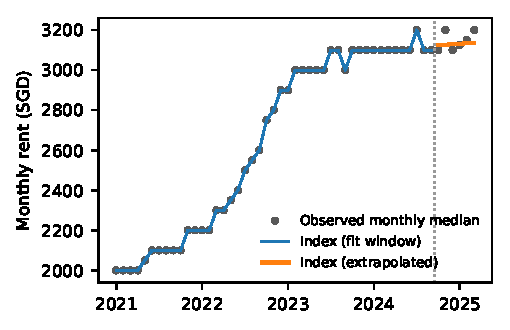
\includegraphics[width=\columnwidth]{figures/rent_index}}
\caption{Monthly median rent and the rent index fitted on January 2021 to September 2024. After the dotted line the index is extrapolated.}
\label{fig:index}
\end{figure}

\begin{table}[htbp]
\caption{Time holdout RMSE (SGD) with the raw target and the index target, G0+G1 features. Change is index minus raw.}
\label{tab:trend}
\centering
\footnotesize
\begin{tabular}{lrrr}
\hline
\textbf{Model} & \textbf{Raw} & \textbf{Index} & \textbf{Change} \\
\hline
Global median & 837.1 & 641.5 & $-195.6$ \\
Group median & 754.9 & 483.1 & $-271.8$ \\
Linear regression & 575.4 & 467.6 & $-107.8$ \\
Ridge & 576.1 & 467.9 & $-108.2$ \\
KNN & 482.3 & 481.9 & $-0.4$ \\
Decision tree & 482.9 & 473.3 & $-9.7$ \\
Random forest & 458.7 & 444.3 & $-14.4$ \\
LightGBM (default) & 457.3 & 454.3 & $-3.0$ \\
CatBoost (default) & 452.7 & 452.2 & $-0.5$ \\
XGBoost (default) & 457.2 & 459.6 & $+2.4$ \\
LightGBM (tuned) & 449.9 & 445.8 & $-4.1$ \\
CatBoost (tuned) & 448.8 & 449.0 & $+0.2$ \\
XGBoost (tuned) & 449.9 & 445.6 & $-4.3$ \\
\hline
\end{tabular}

\end{table}

Table~\ref{tab:trend} shows that the index target lowers the RMSE of 11 of the 13 models. Tuned CatBoost changes by 0.2~SGD. Default XGBoost gets 2.4~SGD worse, but tuned XGBoost gains 4.3~SGD. The gain is largest for the models that cannot represent the rent level well on their own. The global and group medians improve by 196 and 272~SGD, because their raw predictions are medians over all fit months and lie more than 500~SGD below the holdout rents. Linear regression and Ridge improve by 108~SGD. On raw rent they over-predict by 330~SGD on average, because the month coefficient learns the steep rise of 2022 and 2023 and extends it into a period when rents had stopped rising. The other tree models improve by 0 to 14~SGD. They already use the month index to separate recent rows from old ones, but each leaf still averages some older and cheaper rows, so their raw predictions are 28 to 50~SGD too low on average. The index target reduces this bias. With the index target, the untuned random forest (444.3~SGD), tuned XGBoost (445.6~SGD) and tuned LightGBM (445.8~SGD) are the three best models. They lie within 1.5~SGD of each other. The index also removes most of the gap between the simple and the complex models: Ridge falls from 126 to 22~SGD behind LightGBM.

\begin{figure*}[htbp]
\centerline{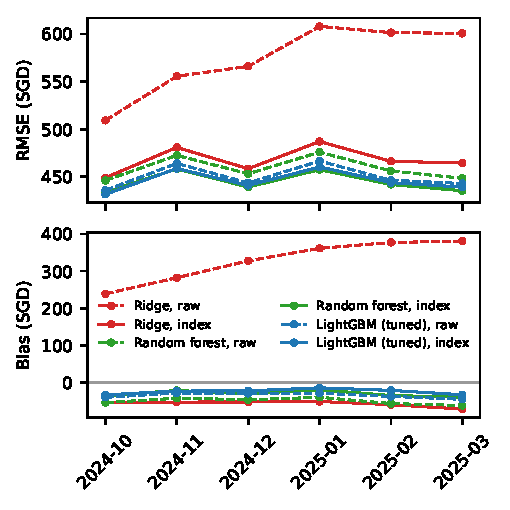
\includegraphics[width=\textwidth]{figures/monthly_rmse}}
\caption{RMSE (left) and bias (right) per validation month for three models, with the raw target (dashed) and the index target (solid).}
\label{fig:monthly}
\end{figure*}

Fig.~\ref{fig:monthly} shows the error per holdout month. For the tree models the error does not grow from October 2024 to March 2025, and the index target lowers it by a similar amount in every month. For Ridge on raw rent the bias grows from 239 to 381~SGD over the six months, which is the expected sign of a wrong trend. Because rents were nearly flat in the holdout period, this holdout cannot show how well a tree model follows a trend that keeps rising. The test period extends up to 16 months past the training data, and only the index target lets a tree model predict a rent level it has not seen. We therefore use the index target for the final model.

\subsection{Models}\label{sec:models}

We compare models in order of complexity, all on the same split and features:
\begin{enumerate}
\item \textbf{Global median} of the fit rows, as a lower bound.
\item \textbf{Group median}: the median rent per town, flat type and calendar quarter. If a group has no fit rows, the lookup falls back to town and flat type, then flat type, then town.
\item \textbf{Linear regression} and \textbf{Ridge} ($\alpha = 10$) with one-hot town, flat type, flat model and subzone. As noted in the progress report, area and flat type are strongly related, so these models keep flat type and drop the area columns.
\item \textbf{$k$-nearest neighbours} ($k = 50$, distance weights) on scaled latitude, longitude, floor area and month.
\item \textbf{Decision tree} (depth 16, at least 20 rows per leaf).
\item \textbf{Random forest}~\cite{breiman2001random} (300 trees, depth 20, at least 5 rows per leaf, 70\% of the features per split).
\item \textbf{LightGBM}~\cite{ke2017lightgbm}, \textbf{CatBoost}~\cite{prokhorenkova2018catboost} and \textbf{XGBoost}~\cite{chen2016xgboost}, gradient boosted trees with native handling of categorical features, first with default settings and then tuned.
\end{enumerate}
The baselines use scikit-learn~\cite{pedregosa2011scikit}. Their settings are fixed and were not tuned.

\subsection{Tuning Budget}

We gave each of the three boosting models a fixed budget of 30 trials of Optuna~\cite{akiba2019optuna} with the tree-structured Parzen estimator~\cite{bergstra2011algorithms}, minimising the time holdout RMSE with G0+G1 features and the raw target. The search covers the number of trees, learning rate, tree size, row and feature subsampling and regularisation (Appendix~\ref{app:hyperparameters}). The tuned settings are then held fixed for the ablations and for the index target. We stopped when the budget ran out, because the course feedback warned against chasing small RMSE gains.

% Owner: member B, with member C for the boosting rows. Target length: 1.5 pages.
% Sources: docs/baseline_results.md, docs/boosting_model_choice.md, results/results.csv.
\section{Evaluation}\label{sec:evaluation}

\todo{Main results table: every model on the time holdout with G0+G1 features. Columns RMSE, MAE, MAPE, bias, fit time. Current numbers: global median 837.1, group median 755.0, linear regression 575.4, Ridge 576.1, KNN 482.3, decision tree 482.9, random forest 458.7, LightGBM default 457.3, CatBoost default 452.7, CatBoost tuned 448.8, LightGBM tuned 449.9, LightGBM tuned with index target 445.8, random forest with index target 444.3. Raw and index results for every model: Table~\ref{tab:trend}.}

\todo{Paragraph on the gaps: how close the lookup and linear models get, and how much boosting adds over the random forest (about 9 to 13 SGD).}

\todo{Feature group ablation table (member C): G0 460--463, G0+G1 449--450, G0+G1+G2 449--450, ALL 450--452. Only the location group helps clearly. The market group hurts slightly.}

\todo{Suspicious row ablation in one sentence: removing the flagged rows does not improve the holdout RMSE.}

\todo{Kaggle public leaderboard score of the final submission, reported as a secondary result.}

% Owner: member D. Target length: 1.25 pages.
\section{Error Analysis and Interpretation}\label{sec:errors}

\todo{Noise floor: group rows with identical features (same block, flat type, area and month) and report the spread of rent within each group. Compare it with the best RMSE.}

\todo{Residuals by town, flat type, rent band, flat age and validation month. Figure~\ref{fig:monthly} already gives the error by month.}

\todo{The 20 largest errors, grouped by cause: data error, missing attribute or rare segment.}

\todo{Permutation importance or SHAP for the final model, and partial dependence for area, age, MRT distance and month. Compare with the Spearman ranking from Section~\ref{sec:data}.}

\todo{What the boosting model learns that Ridge misses.}

% Owner: all members. Target length: 0.5 page.
\section{Limitations and Future Work}\label{sec:limitations}

The data does not record the floor of the unit, its condition or furnishing, or whether the whole flat or only some rooms are rented. These attributes explain part of the rent that no model in this report can recover.

Our holdout covers six months of flat rents, while the test period extends up to 16 months past the training data. To test the trend handling under other conditions, we moved the end of the fit window back and forecast 16 months ahead from four earlier dates (Table~\ref{tab:horizon}). The index target helps while rents keep rising: fitted to March 2022, LightGBM scores 762~SGD against 909~SGD raw on months 7 to 16. It hurts when they stop: fitted to March 2023, the line through the last 12 medians still rises by 70~SGD per month, and LightGBM scores 955~SGD against 569~SGD raw, with a bias of $+743$~SGD. The index is therefore a bet that the recent slope continues. For the final model the slope is only 5.3~SGD per month, so the index reaches SGD~3{,}246 at the end of the test period against a last observed median of SGD~3{,}200. This limits the risk, but errors on the test set are likely larger than on the holdout, especially if the rent trend changes direction.

The market features (COE, CPI and stock values) use the value of the approval month, which would not be known when a future rent is predicted. They did not improve the holdout RMSE, and the final model does not use them.

\todo{Data we did not integrate: rents by market segment, work pass counts, BTO completion schedules, travel times, unit storey.}


\bibliographystyle{IEEEtran}
\bibliography{references}

\appendices
% Appendix: not counted in the 8 page limit.
\section{Workload}\label{app:workload}

\todo{Required workload table: one row per member with the tasks they did.}

\section{Forecast Backtest}\label{app:backtest}

\begin{table}[htbp]
\caption{RMSE (SGD) when the fit window ends earlier, by months ahead, G0+G1 features. Hyperparameters are the final ones, so these runs borrow some information from later data.}
\label{tab:horizon}
\centering
\footnotesize
\begin{tabular}{llrrrrrr}
\hline
 & & \multicolumn{2}{c}{\textbf{LightGBM}} & \multicolumn{2}{c}{\textbf{XGBoost}} & \multicolumn{2}{c}{\textbf{Forest}} \\
\textbf{Fit to} & \textbf{Months} & Raw & Index & Raw & Index & Raw & Index \\
\hline
2022-03 & 1--6 & 535 & 517 & 536 & 512 & 552 & 509 \\
2022-03 & 7--16 & 909 & 762 & 912 & 758 & 937 & 756 \\
2022-09 & 1--6 & 698 & 652 & 711 & 648 & 731 & 649 \\
2022-09 & 7--16 & 727 & 622 & 741 & 614 & 768 & 609 \\
2023-03 & 1--6 & 640 & 668 & 632 & 661 & 669 & 666 \\
2023-03 & 7--16 & 569 & 955 & 562 & 946 & 589 & 954 \\
2023-09 & 1--6 & 557 & 577 & 550 & 574 & 559 & 566 \\
2023-09 & 7--16 & 491 & 598 & 486 & 593 & 496 & 574 \\
2024-03 & 1--6 & 496 & 492 & 492 & 492 & 501 & 494 \\
2024-03 & 7--16 & 455 & 451 & 452 & 450 & 462 & 449 \\
\hline
\end{tabular}

\end{table}

\section{Hyperparameters}\label{app:hyperparameters}

\begin{table}[htbp]
\caption{Final hyperparameters. Models not listed use the library defaults with seed 5228.}
\label{tab:hyperparameters}
\centering
\footnotesize
\begin{tabular}{p{0.24\columnwidth}p{0.66\columnwidth}}
\hline
\textbf{Model} & \textbf{Settings} \\
\hline
Ridge & alpha = 10 \\
KNN & k = 50, distance weights \\
Decision tree & depth 16, 20 rows per leaf \\
Random forest & 300 trees, depth 20, 5 rows per leaf, max features 0.7 \\
LightGBM (tuned) & n\_estimators = 500, learning\_rate = 0.0344, num\_leaves = 205, min\_child\_samples = 51, feature\_fraction = 0.896, bagging\_fraction = 0.914, bagging\_freq = 1, reg\_alpha = 0.0697, reg\_lambda = 0.00147 \\
CatBoost (tuned) & iterations = 2000, learning\_rate = 0.0487, depth = 9, l2\_leaf\_reg = 11.3, random\_strength = 0.039, subsample = 0.539 \\
XGBoost (tuned) & n\_estimators = 1100, learning\_rate = 0.0109, max\_depth = 9, min\_child\_weight = 2.94, subsample = 0.781, colsample\_bytree = 0.516, reg\_alpha = 0.00331, reg\_lambda = 1.57 \\
\hline
\end{tabular}

\end{table}


\end{document}
